\section{Smart meter privacy concerns}\label{smart_meter_privacy}
The consumption data collected by a smart meter can be fine-grained.
This fine-grained data means that sensitive knowledge about the consumer can be obtained.
The following describes how one can obtain and use this knowledge, which is based on \citet{privacy_memoir}.
\mikael{I think there should be something about how this knowledge about the consumer could be exploited.}

\subsection{Experiment}
The setting, in which is collected sixty days of power consumption data from three households, consists of the following physical components:
\begin{itemize}
\item TED energy monitor
\item SheevaPlug
\end{itemize}
The energy monitor is connected to the two incoming electricity phases, A and B.\cite{TED_installation_guide}
The SheevaPlug is connected to the router, and the energy monitor, and is used to access the data remotely.
The energy monitor returns a tuple $(t,p)$ where $t$ is the time and $p$ is the power-usage since last measurement.
The power is measured every second, so we have a tuple for every second with the power used the past second.
Finally, the three households are to make a "power activity"-journal for a minimum of three days.
In this journal they write down when they turn on and off any electric devices.

When the data is collected it is analysed in four steps:
\begin{itemize}
\item Pre-process data
\item Tag power events
\item Filter out automated appliances
\item Map consumption events to real life events
\end{itemize}

\paragraph{Pre-process data}
The data is pre-processed using DBSCAN, which is a density-based clustering algorithm.
This helps group power tuples into power segments, where a power segment is a collection of power tuples with a pattern adjacent in time.
Each power segment then gets tagged with a label, start time, average power usage, duration, beginning power step, and a shape label.

\paragraph{Tag power events}
In \cref{consumption_one_day} we are able to see the consumption data for one household after the second step of the analysis.
On the x-axis we have time in hours, for an entire 24-hour period, and on the y-axis we have power usage in kWh.
Already at this stage of the analysis we are able to say something about when there is activity in the household.
We can also see how there are some automated appliances that are on all the time or at certain intervals.
We can determine this by assuming there is almost no activity in the night, and by collecting data over several days.

\begin{figure}
  \begin{center}
    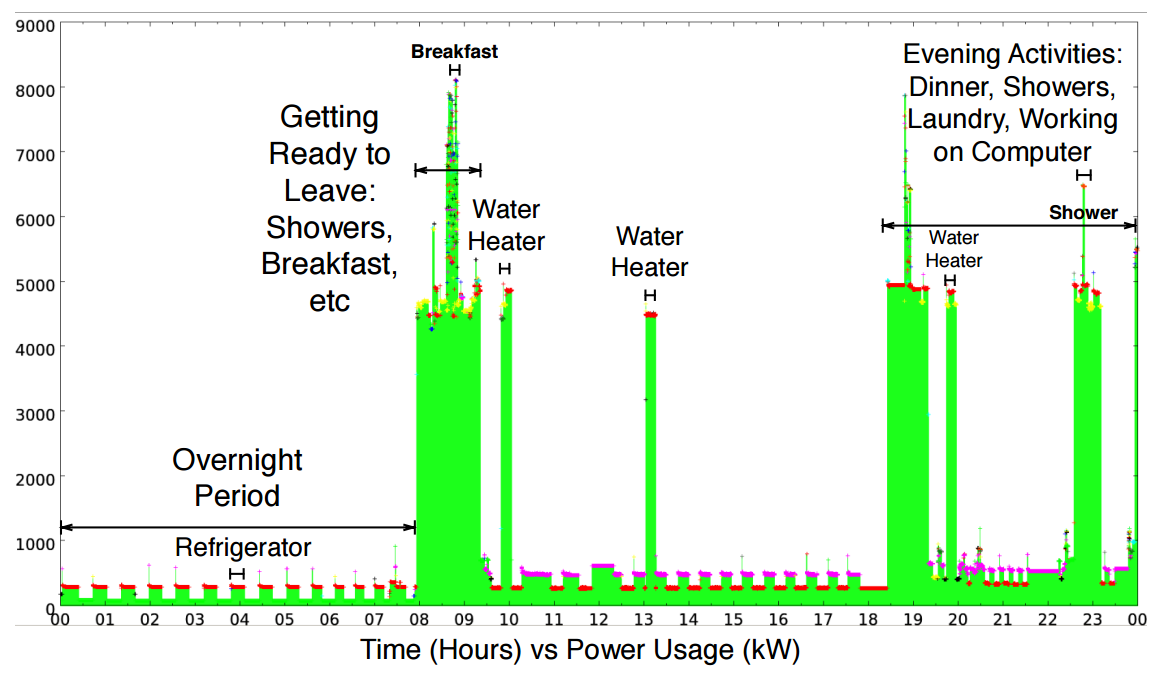
\includegraphics[width=\textwidth]{consumption_one_day.png}
  \end{center}
  \caption{A day of consumption data after the second step of analysis, labelled with real life events -- taken from the power activity journal.}
  \label{consumption_one_day}
\end{figure}

\paragraph{Filter out automated appliances}
The third step is to filter out automated appliances, such as the refrigerator (see \cref{consumption_one_day}).
This is done by looking at the consumption data and reason about whether the power usage is from a human interaction or not.
If, for instance, the distinct usage also occurs at night, it is probably an automated appliance and by looking at a lot of data one can be rather certain.
At last the power segments are labelled corresponding to real time events, by looking at the power activity journals.

\paragraph{Map consumption events to real life events}
In \cref{detailed_consumption} we can see how the consumption for a small time period looks like after all four steps of the analysis.
At this point it is pretty easy to say something about what kind of activities are going on.
The time period is for a typical morning where we can see the household uses the stove, coffee maker, toaster, and some computer screens.

\begin{figure}
  \begin{center}
    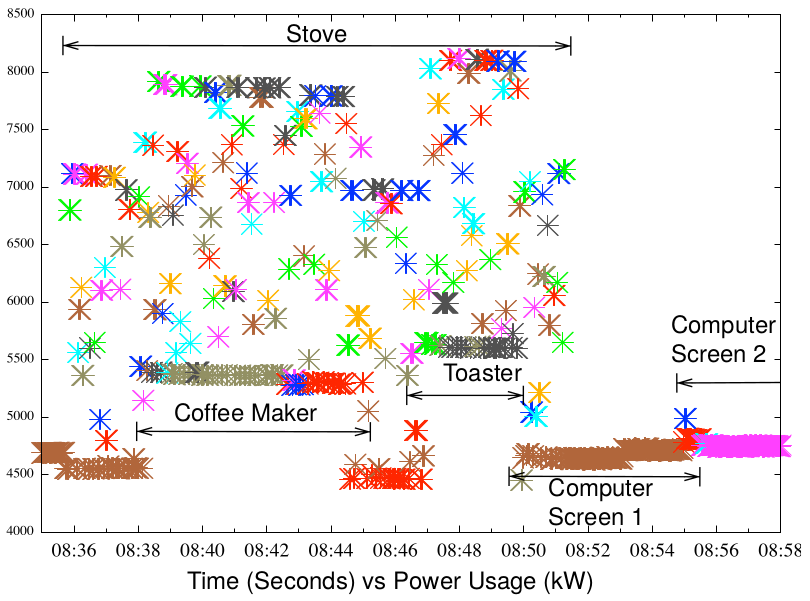
\includegraphics[width=\textwidth]{detailed.png}
  \end{center}
  \caption{Power consumption data after all four steps of the analysis for a small time period -- a morning when the household is getting breakfeast, etc.}
  \label{detailed_consumption}
\end{figure}

As we can see by this example, when collecting only a small amount of consumption data and doing trivial analysis, it is possible to say a lot about a household.
Utilities companies or similar, that have access to much more data, can learn even more by using their combined knowledge. \stefan{what is it they have that can provide more information?}

\subsection{Privacy issues}\label{privacy_concerns}
As it can be seen in the previous section, it is possible to determine a lot about a household, simply based on power consumption.
This can lead to privacy issues, where some of these issues are described in the following

\paragraph{Amount of people home}
When having a lot of consumption data one can determine the amount of people who are home and begin to see patterns in the power usage and map that to people.
This means that over time it is possible to determine \textit{who} is home, where \textit{who} can be seen as a power usage pattern for a person in the household.

\paragraph{Household activities}
  
It is also possible to say a lot about household activities, even with a small amount of consumption data.
For instance, we can begin to reason about if a household had a good nights sleep, or if the household was eating hot or cold breakfast.
And even if the household was watching a specific sport event last night.
\paragraph{Information about appliances}
By extending the analysis one could look for specific appliance signatures in the power trace and from this say some more about the household \cite{NILM}.
